\chapter{System Overview}
\label{chap:system-overview}

The system being specified is the Thermostat of an Isolette.\footnote{To simplify this example, the Operator Interface is treated as an external entity outside of the Thermostat.}  An Isolette is an incubator for an Infant that provides controlled temperature, humidity, and oxygen (if necessary). Isolettes are used extensively in Neonatal Intensive Care Units for the care of premature infants.

The purpose of the Isolette Thermostat is to maintain the air temperature of an Isolette within a desired range. It senses the Current Temperature of the Isolette and turns the Heat Source on and off to warm the air as needed. If the temperature falls too far below or rises too far above the Desired Temperature Range, it activates an alarm to alert the Nurse. The system allows the Nurse to set the Desired Temperature Range and to set the Alarm Temperature Range outside the Desired Temperature Range of which the alarm should be activated.

\section{System Content}
\label{sec:system-content}

The operational context of the Isolette Thermostat is shown in Figure~\ref{fig:state-concepts}.

%% import image
\begin{figure*}[ht]
  \centerline{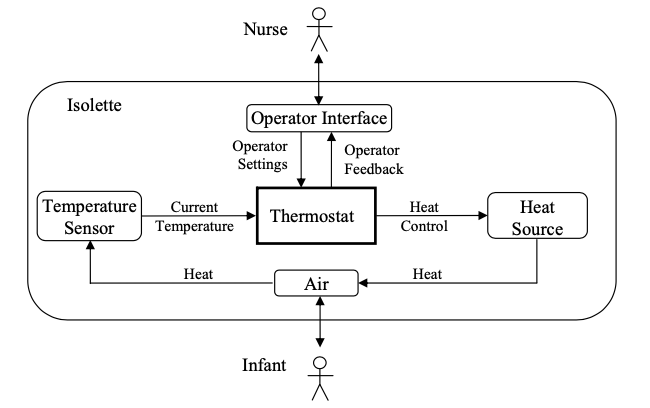
\includegraphics[width=\textwidth]{figures/thermostat-context-diagram.png}}
  \vspace{-.4cm}
  \caption{Context Diagram for the Isolette Thermostat}
  \vspace{-.4cm}
 \label{fig:state-concepts}
\end{figure*}


The Thermostat interacts directly with three entities that are part of the Isolette:
\begin{itemize}
\item The Temperature Sensor provides the Current Temperature of the air in the Isolette to the Thermostat.
\item The Heat Source heats the Air in the Isolette. It is turned on and off by the Heat Control.
\item The Operator Interface provides the Operator Settings for the Thermostat and receives Operator Feedback from the Thermostat.
\end{itemize}

The Thermostat also interacts indirectly with other entities outside of the Isolette:
\begin{itemize}
\item The Nurse who uses the Operator Interface to enter the Operator Settings and view the Operator Feedback.
\item The Air in the Isolette.
\item The Infant that is placed in the Isolette and is warmed by the Air.
\end{itemize}

\section{System Goals}
\label{sec:system-goals}

The high-level goals (G) of the system are:
\begin{itemize}
  \item G1—The Infant should be kept at a safe and comfortable temperature.
  \item G2—The Nurse should be warned if the Infant becomes too hot or too cold.
  \item G3—The cost of manufacturing the Thermostat should be as low as possible.
\end{itemize} 

